%%%%%%%%%%%%%%%%%%%%%%%%%%%%%%%%%%%%%%%%%%%%%%%%%%%%%%%%%%%%%%%%%%%%%%%%%%%%%%%%
%  Single-column LaTeX Template with IST Logo and Modular Inputs
%  Author: João Pires
%  Instituto Superior Técnico, Lisboa
%%%%%%%%%%%%%%%%%%%%%%%%%%%%%%%%%%%%%%%%%%%%%%%%%%%%%%%%%%%%%%%%%%%%%%%%%%%%%%%%

\documentclass[12pt,a4paper]{article}

% =====================================================================
% PACKAGES
% =====================================================================
\usepackage[margin=1in]{geometry}     % 1 inch margins
\usepackage{graphicx}                 % figures (for logo and plots)
\usepackage{caption}
\usepackage{subcaption}
\usepackage{amsmath, amssymb, amsfonts}
\usepackage{booktabs}                 % professional tables
\usepackage{float}                    % precise figure placement
\usepackage{titlesec}                 % control section spacing
\usepackage{indentfirst}              % indent first paragraph
\usepackage{setspace}
\usepackage[numbers,sort&compress]{natbib}
\usepackage{hyperref}
\usepackage{xcolor}
\usepackage{fancyhdr}

% =====================================================================
% STYLE SETTINGS
% =====================================================================
\hypersetup{
	colorlinks=true,
	linkcolor=black,
	citecolor=blue!60!black,
	urlcolor=blue!70!black
}

% --- 
%\newcommand{\sectionbreak}{\clearpage}
% --------------------------------

% section formatting
\titleformat{\section}{\normalfont\bfseries\large}{\thesection.}{0.5em}{}
\titleformat{\subsection}{\normalfont\bfseries\normalsize}{\thesubsection.}{0.5em}{}

\titlespacing*{\section}{0pt}{1em plus .2em minus .1em}{0.5em}
\titlespacing*{\subsection}{0pt}{0.8em plus .2em minus .1em}{0.4em}

\captionsetup[subfigure]{labelfont=bf,textfont=normalfont}
\captionsetup[figure]{labelfont=bf}
\captionsetup[table]{labelfont=bf}


% Header/Footer (opcional — remove se não quiseres nada no topo/rodapé)
%\pagestyle{fancy}
%\fancyhf{}
%\fancyhead[L]{Revisiting K-core robustness}
%\fancyhead[R]{João Pires — IST, 2025}
%\fancyfoot[C]{\thepage}

% =====================================================================
% TITLE BLOCK
% =====================================================================
\title{
	\vspace{-2.5cm} % move logo e título para cima
	
\includegraphics[width=3.5cm]{Figures/logo_ist.png}\\[0.5cm]
	\bfseries Computational Statistics Practical Report-5 \\
	\Large 2025/2026
	\vspace{-0.4cm}
}


\author{
	João Pires (ist1116478) and Gustavo Brazil (ist1116490) \\[0.1em]
	\normalsize Instituto Superior Técnico, University of Lisbon, Portugal\\
	\vspace{-0.8cm}
}

\date{January 9th, 2026}

%\vspace{-3cm}

% Alargar o texto do abstract mantendo o título centrado como está
% Alargar o texto do abstract e reduzir o espaço após a data
\makeatletter
\renewenvironment{abstract}{
	\vspace{-2em} % 🔧 ajusta a distância entre a data e o título "Abstract"
	\begin{center}
		{\bfseries \abstractname\vspace{0.06cm}} % título centrado
	\end{center}
	\list{}{%
		\setlength{\leftmargin}{0pt}%
		\setlength{\rightmargin}{0pt}%
	}%
	\item\relax
}{\endlist\vspace{0.5em}}
\makeatother



% Ajustar o ambiente abstract para ter a mesma largura que o texto normal
%\makeatletter
%\renewenvironment{abstract}{
	%	\vspace{1em}
	%	\noindent\textbf{\abstractname.}\quad
	%}{\par\vspace{1em}}
%\makeatother

% =====================================================================
% DOCUMENT
% =====================================================================

%\renewcommand{\thesection}{Chapter \arabic{section}}
\usepackage{tabularx}

% --- Adicionar ao Preâmbulo (antes de \begin{document}) ---
\usepackage{listings}
\usepackage{xcolor}
\usepackage{caption} % <--- ADICIONAR ESTE PACOTE

% Configuração para tornar o rótulo (ex: "Listing 1") em negrito
\captionsetup[lstlisting]{labelfont=bf}

% A tua configuração original (mantida igual)
\lstset{ 
	language=R,                     % Linguagem R
	basicstyle=\footnotesize\ttfamily, % Fonte pequena e monoespaçada
	numbers=left,                   % Números na esquerda
	numberstyle=\tiny\color{gray},  % Estilo dos números
	stepnumber=1,                   % Numerar todas as linhas
	numbersep=5pt,                  % Distância dos números
	backgroundcolor=\color{white},  % Fundo branco
	showspaces=false,               % Não mostrar espaços
	showstringspaces=false,         % Não mostrar espaços em strings
	showtabs=false,                 % Não mostrar tabs
	frame=single,                   % Moldura à volta do código
	rulecolor=\color{black},        % Cor da moldura
	tabsize=2,                      % Tamanho do tab
	captionpos=b,                   % Posição da legenda (bottom)
	breaklines=true,                % Quebrar linhas longas
	breakatwhitespace=false,        % Quebrar apenas em espaços?
	title=\lstname,                 % Mostrar o nome do ficheiro (opcional)
	keywordstyle=\color{blue},      % Keywords em azul
	commentstyle=\color{teal},      % Comentários em verde escuro
	stringstyle=\color{violet},     % Strings em roxo
	escapeinside={\%*}{*)},         % Se quiser adicionar LaTeX dentro do código
	morekeywords={*,...}            % Adicionar keywords extra se necessário
}


\begin{document}
	
	\maketitle
	\thispagestyle{plain}
	
	%\vspace{-1cm}
	
	
	% ================================================================
	% Modular file structure (each section in its own .tex file)
	% ================================================================
	\vspace{-1cm}
	\section{Introduction}
The primary objective of this practical report is to investigate the relationship between Glycosolated Hemoglobin (GHB) and a set of physiological risk factors in a sample of African American subjects from central Virginia, as originally presented by Faraway \cite{farway2016}. GHB is an important marker for diabetes diagnosis, where levels above 7.0 typically indicate a positive diagnosis. Given the continuous and strictly positive nature of the response variable (GHB), combined with the right-skewness of the biological data, standard linear regression models (such as Ordinary Least Squares), which assume normality (Gaussian distribution), may be inappropriate. Therefore, this report proposes a Generalized Linear Model (GLM) assuming a Gamma distribution with a log-link function.

Our analysis follows a Bayesian perspective, utilizing Markov Chain Monte Carlo (MCMC) methods for parameter estimation, followed by model selection based on the Deviance Information Criterion (DIC). Finally, to ensure the robustness of the findings and satisfy the requirement for innovation, the results are validated using a non-parametric Bootstrap approach.
	\section{Exploratory Data Analysis (EDA)}
The original dataset comprises data from 390 subjects. However, some of them have missing values in some variables. Since the proposed Bayesian model requires complete cases for all predictors, a data cleaning process was performed by removing observations with incomplete entries. As a result, the effective sample size used for this analysis consists of 367 subjects (approximately 94\% of the original sample). The response variable is GHB, and the potential predictors include Stabilized Glucose (SGLU) among others. All statistical analyses and visualisations were conducted using R programming language \cite{rstat}.

\begin{figure}[h!]
	\centering
	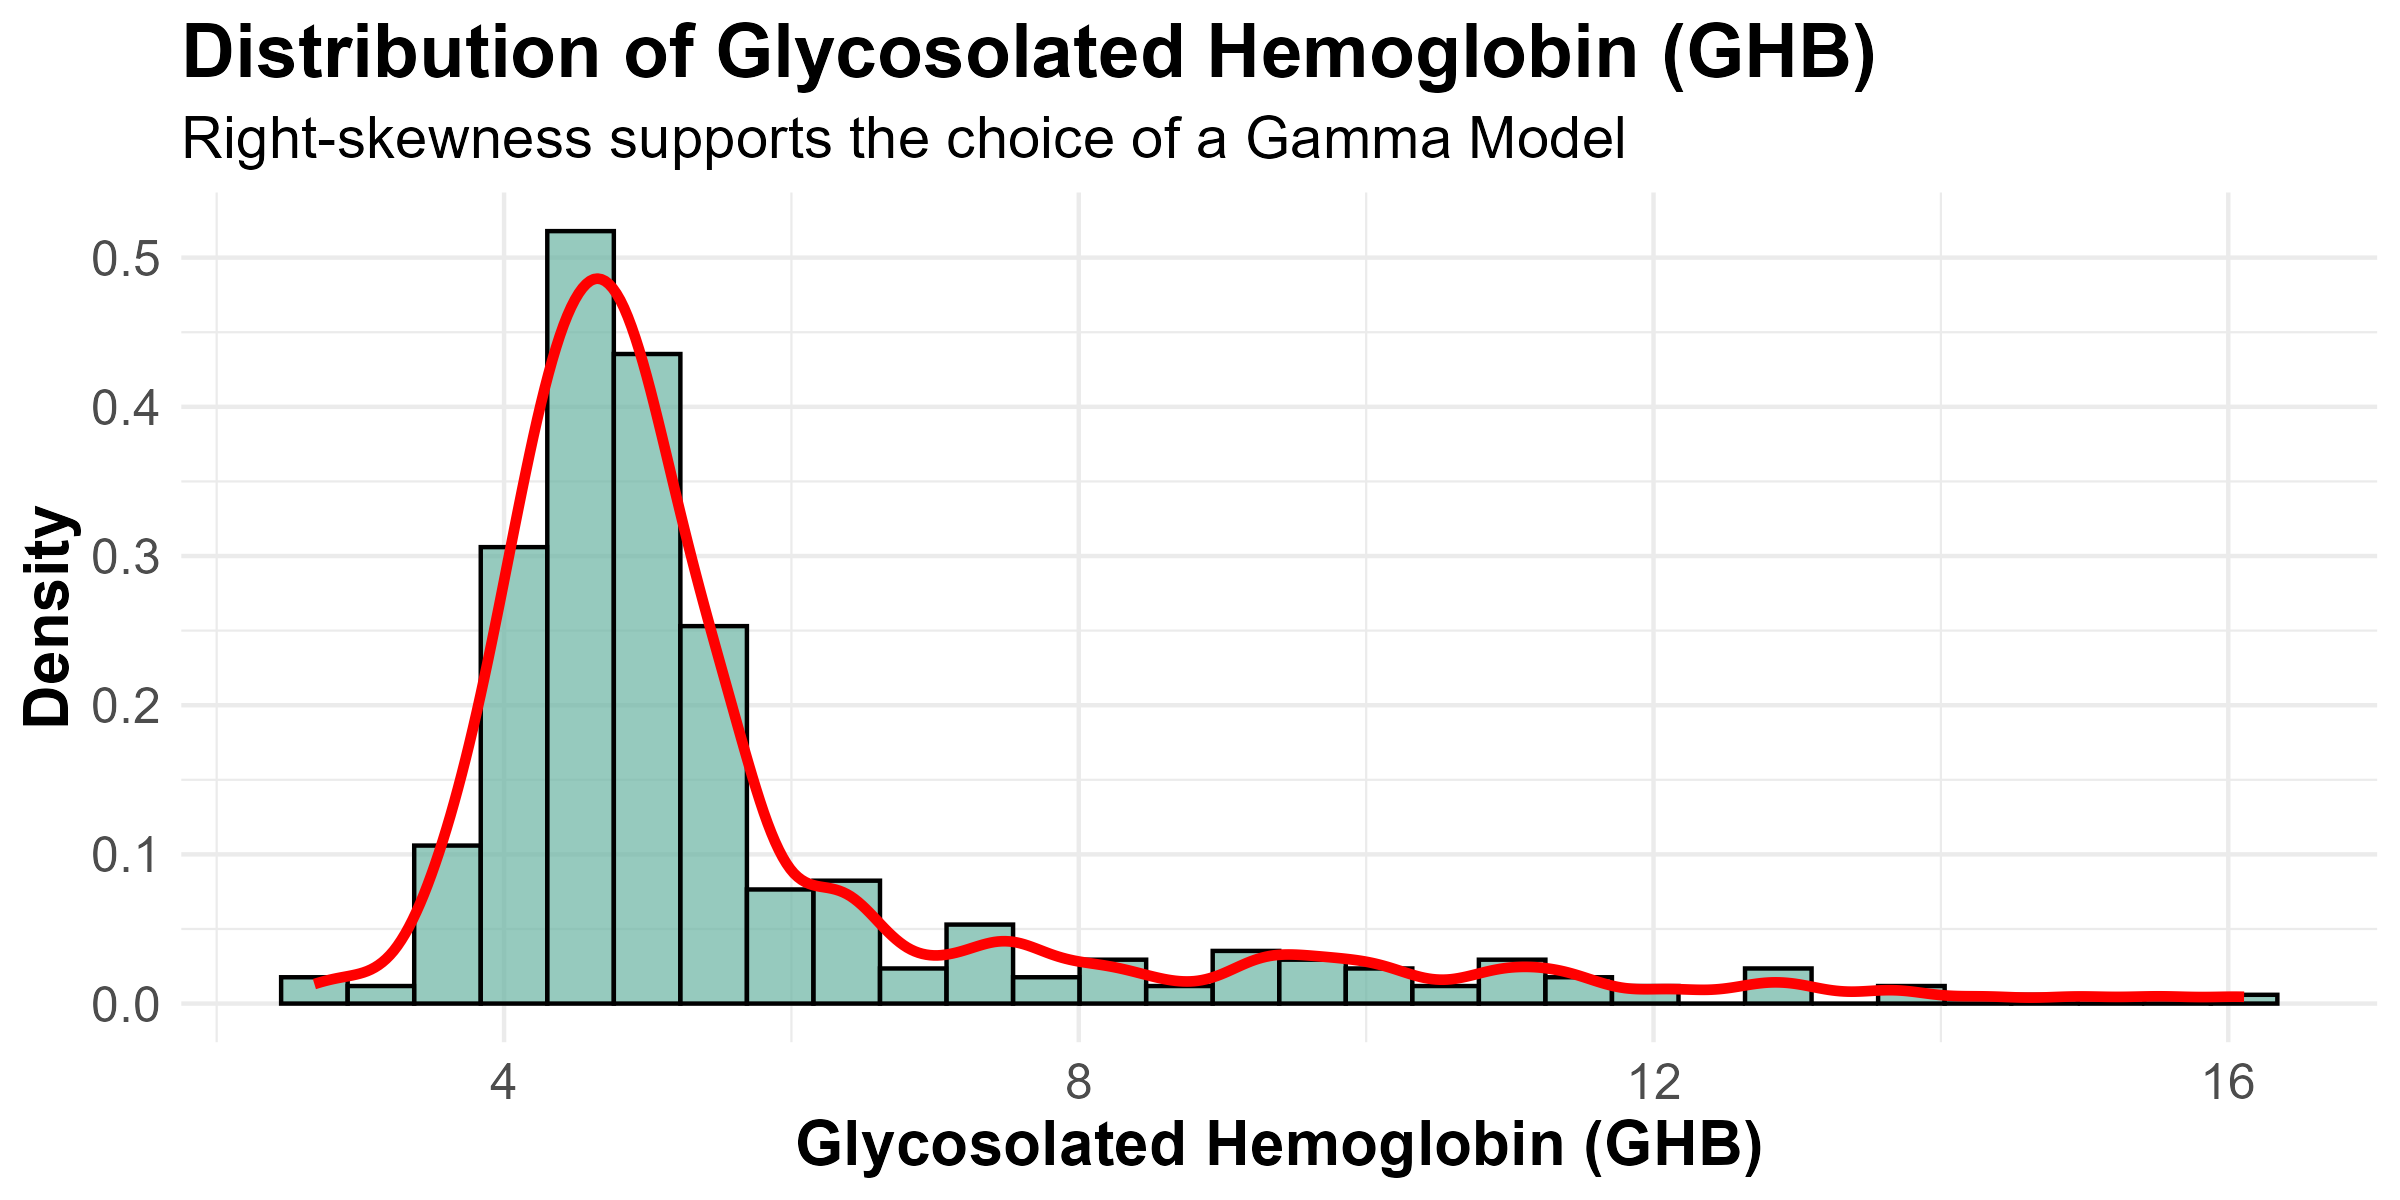
\includegraphics[width=0.63\linewidth]{Figures/histogram_ghb}
	\caption{Histogram and density estimate of GHB levels.}
	\label{fig:histogramghb}
\end{figure}
As observed in Figure (\ref{fig:histogramghb}), the distribution of GHB is asymmetric with a long right tail (positive skewness), with only positive values. This observation confirms that a Normal distribution would be a poor fit for the data and supports the choice of a Gamma distribution, which is ideal for modeling continuous, positive, and skewed data \cite{silva2023notes}.
\begin{figure}[h!]
	\centering
	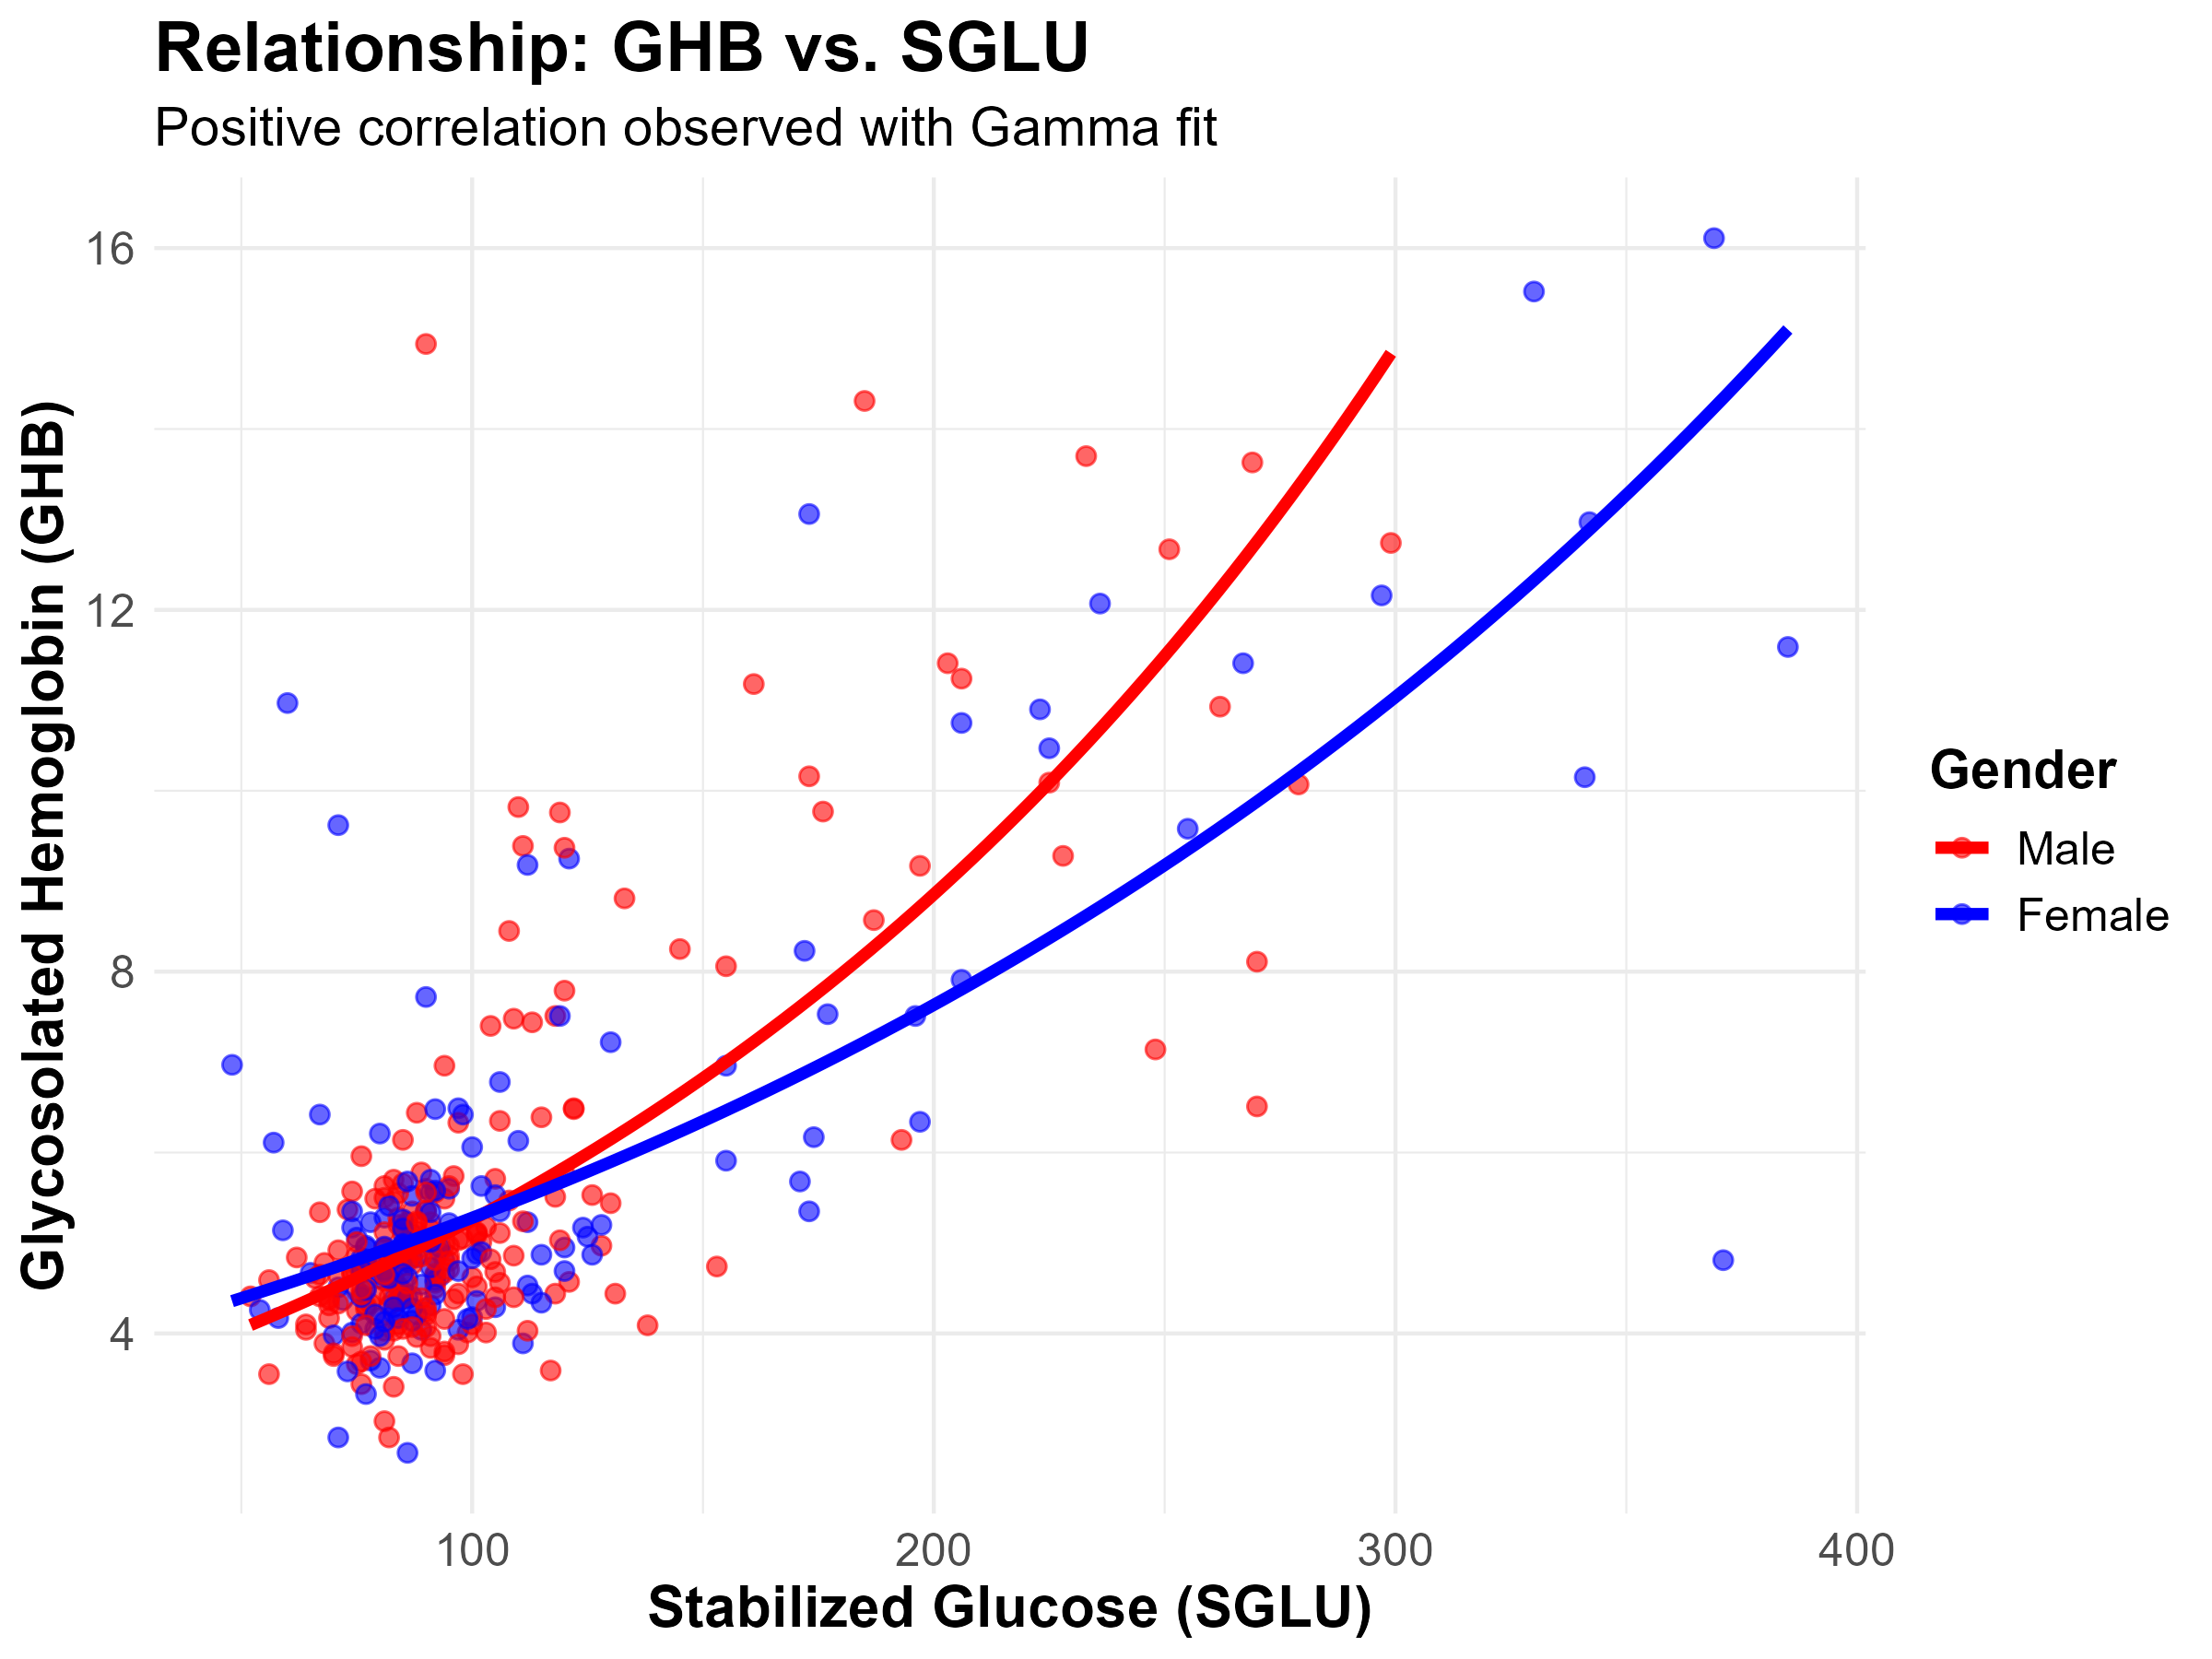
\includegraphics[width=0.54\linewidth]{Figures/scatterplot_glucose}
	\caption{Scatter plot of GHB against SGLU, stratified by gender.}
	\label{fig:scatterplotglucose}
\end{figure}

Figure (\ref{fig:scatterplotglucose}) illustrates the relationship between GHB and SGLU. There is a visible positive trend: as glucose levels increase, GHB levels also tend to rise. This suggests that SGLU will likely be a significant predictor in our regression model. No obvious clustering was found regarding the Location variable (Buckingham vs. Louisa), suggesting geographic factors might not be significant. Although the plot distinguishes between male and female subjects, the fitted regression curves for both groups appear to follow a very similar trajectory/slope. 

\begin{figure}[h!]
	\centering
	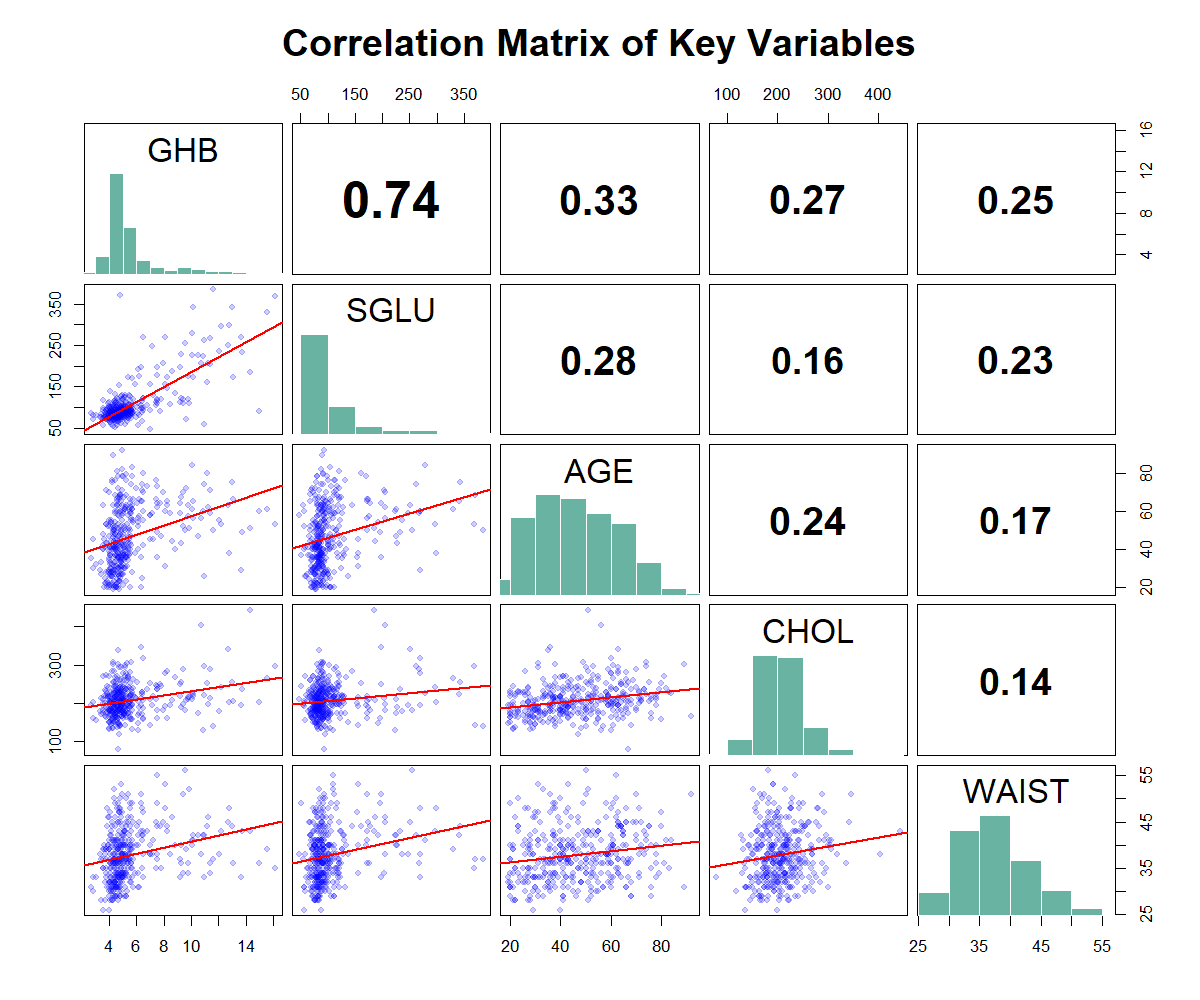
\includegraphics[width=0.65\linewidth]{Figures/correlation_matrix_final_large}
	\caption{Matrix of pairwise scatter plots, histograms, and Pearson correlation coefficients for the response variable (GHB) and key predictors.}
	\label{fig:correlationmatrixfinallarge}
\end{figure}

To investigate multicollinearity and secondary predictors, a Pearson correlation matrix was generated (Figure (\ref{fig:correlationmatrixfinallarge})). To avoid ambiguity with the Gamma shape parameter ($r$), we denote the sample correlation coefficient as $c$. Based on the multivariate analysis, a selection criterion was established to retain predictors showing a correlation of at least 0.20 ($c \ge 0.20$) with the response variable. Applying this threshold, the following variables were selected for the Bayesian regression model: SGLU, Age, Cholesterol, Waist Circumference and Systolic Blood Pressure (SBP) (the full correlation matrix (Appendix (\ref{app:apexA})) confirms that SBP also meets the inclusion threshold). This data-driven selection ensures that the model focuses on factors with meaningful associations with GHB.

\begin{figure}[h!]
	\centering
	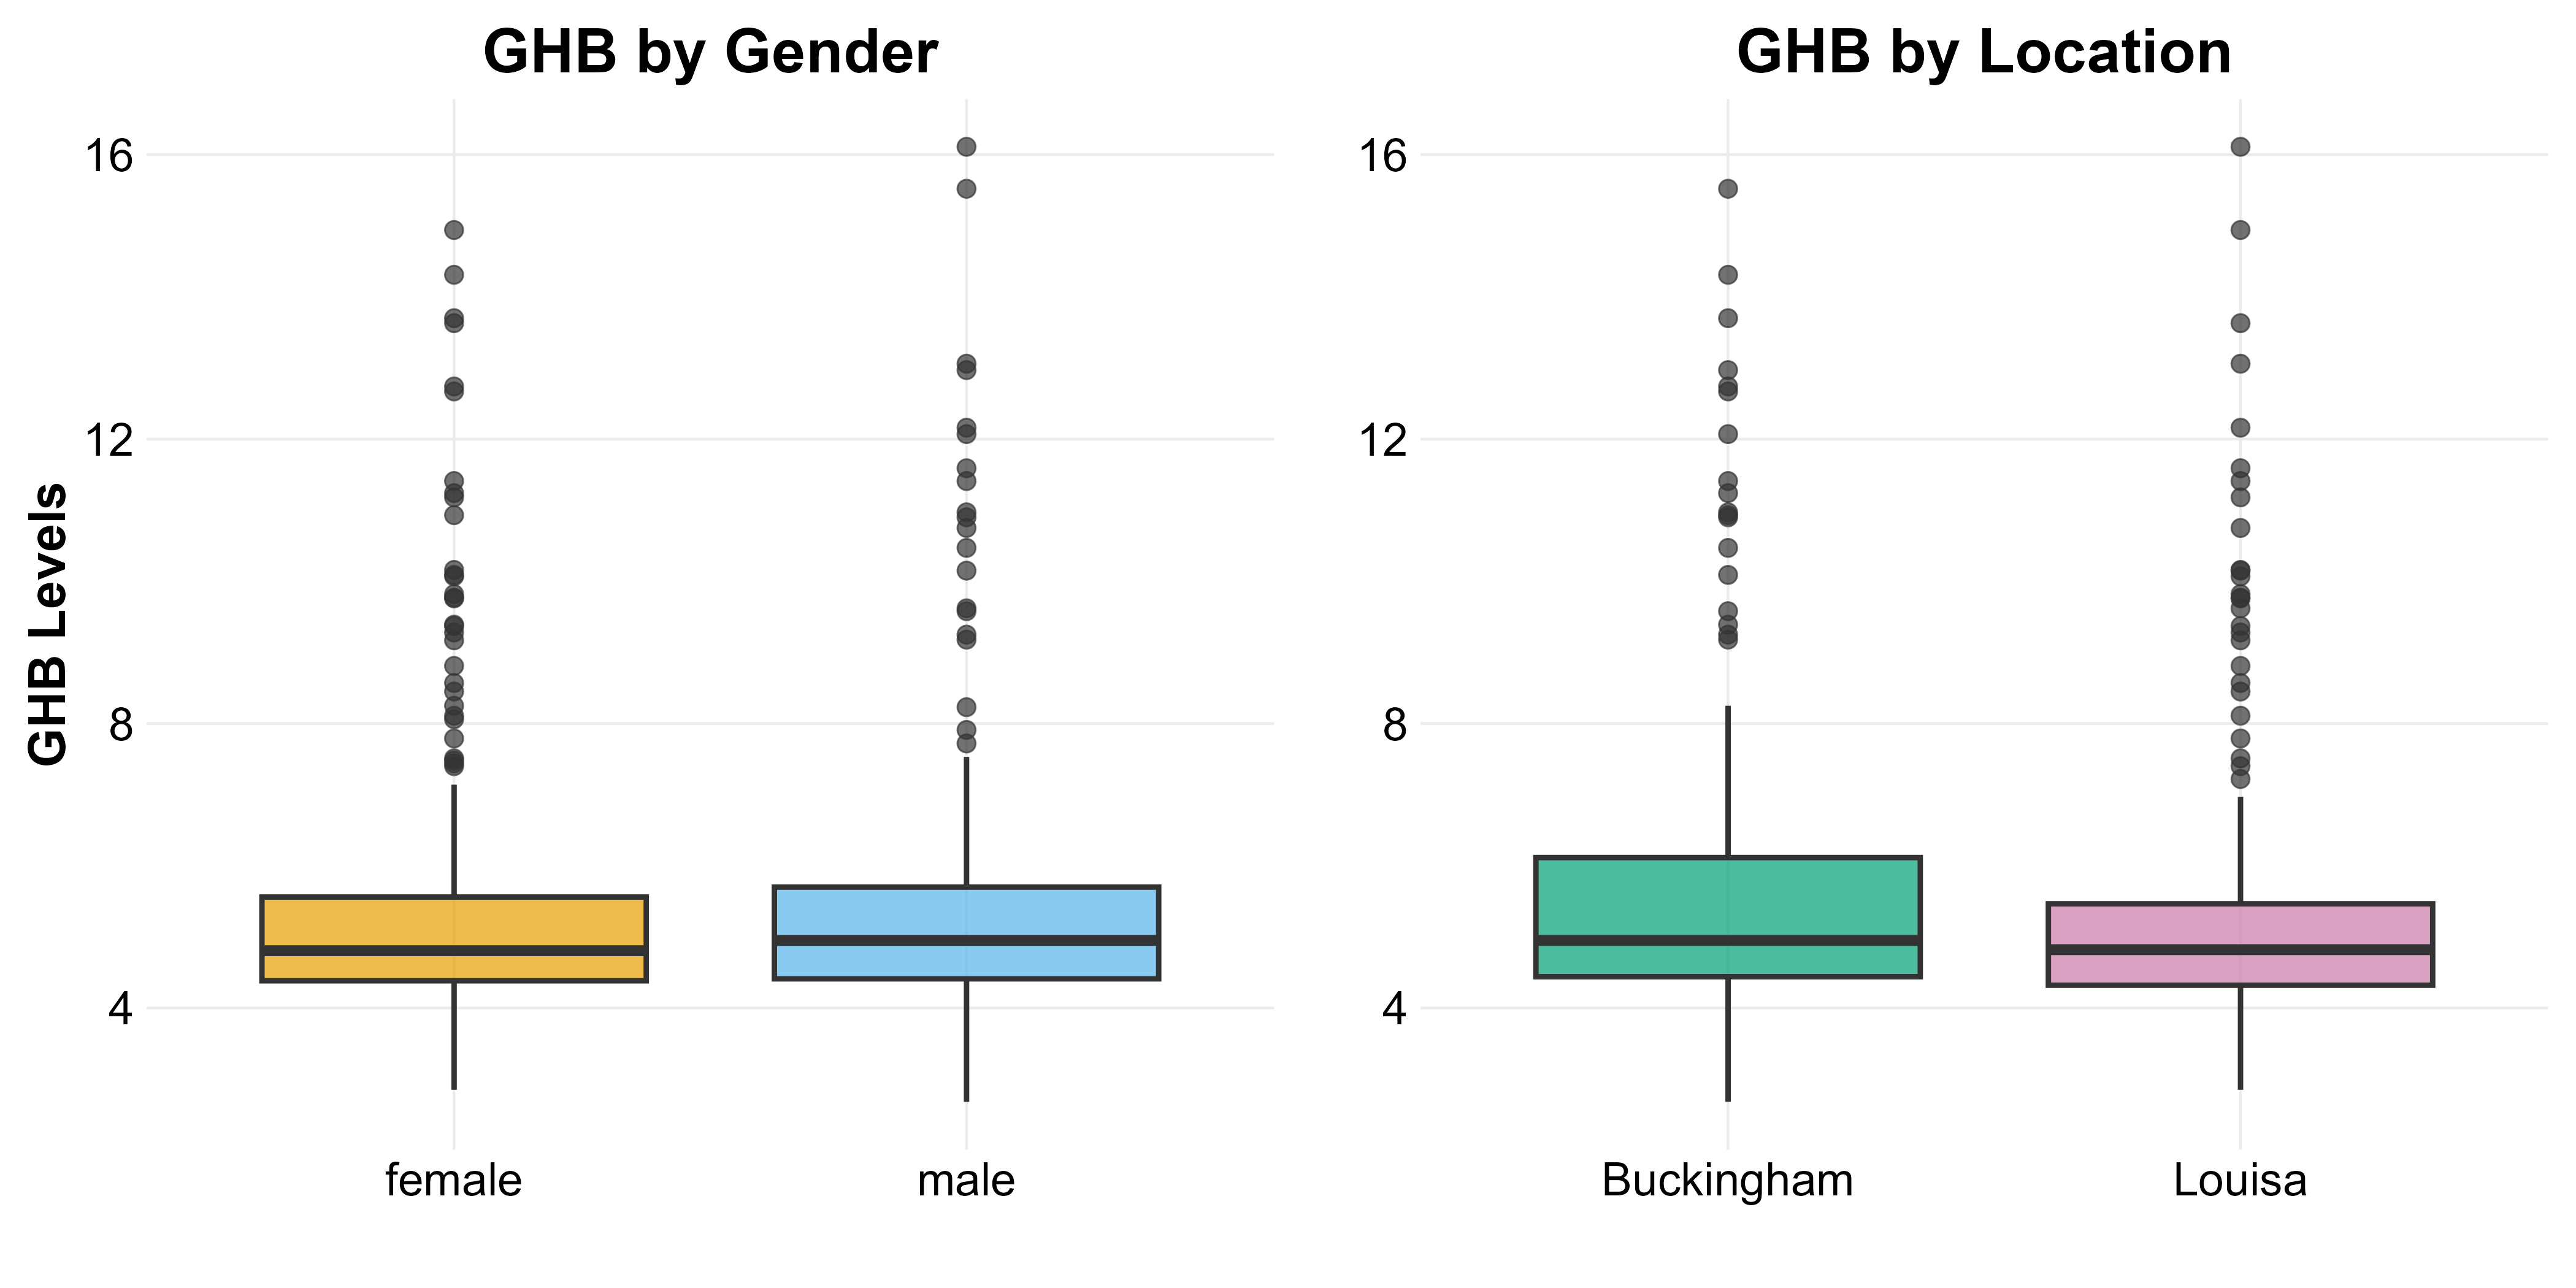
\includegraphics[width=0.7\linewidth]{Figures/boxplots_categorical}
	\caption{Boxplots of GHB levels stratified by demographic factors: Gender (left) and Location (right).}
	\label{fig:boxplotscategorical}
\end{figure}
To assess the potential impact of demographic factors, we analyzed the distribution of GHB across Gender and Location using boxplots (Figure (\ref{fig:boxplotscategorical})). The median GHB levels are very similar for females and males. The interquartile ranges also show significant overlap, suggesting that gender is not a strong differentiator. Similarly, the distribution of GHB levels appears consistent between subjects from Buckingham and Louisa. Both plots reveal the presence of high-value outliers, indicating subjects with severe diabetic conditions across all demographic groups. Neither gender nor location are primary driver of GHB levels.






	\section{The Bayesian Generalized Linear Model}
Given that the response variable $y_i$ (GHB) is continuous, strictly positive, and right-skewed, we assume that the observations $y_i$ are independently distributed according to a Gamma distribution \cite{silva2023notes}. The model is parameterized in terms of the mean $\mu_i$ and a shape parameter $r$. The probability density function is defined as: 

\begin{equation*}	
	y_i \sim \text{Gamma}(r, \lambda_i).
\end{equation*}

Where the rate parameter is $\lambda_i = r / \mu_i$, such that $E[y_i] = \mu_i$ and $Var(y_i) = \mu_i^2 / r$. To map the linear predictor to the positive mean $\mu_i$, we employ the Log-Link function: 

\begin{equation*}	
	\log(\mu_i) = \eta_i.
\end{equation*}

Based on the variable selection performed in the EDA section (variables with correlation $c \ge 0.20$), the linear predictor $\eta_i$ for subject $i$ is defined as:
\begin{equation*}
	\eta_i = \beta_0 + \beta_{SGLU} \cdot \text{SGLU}_i + \beta_{AGE} \cdot \text{AGE}_i + \beta_{CHOL} \cdot \text{CHOL}_i + \beta_{WAIST} \cdot \text{WAIST}_i + \beta_{SBP} \cdot \text{SBP}_i.
\end{equation*}

Where $\beta_0$ represents the intercept and $\beta_k$ represents the regression coefficient for each predictor. Following the Bayesian framework, we must specify prior distributions for all unknown parameters. Since no strong prior information was available for this specific population, we adopted vague (non-informative) priors to allow the data to dominate the posterior distribution \cite{gelman2013}. We assigned Normal priors with mean 0 and low precision ($\tau=0.001$, implying a variance of $\sigma^2 = 1000$) to represent our initial uncertainty: 
$$\beta_k \sim N(\mu=0, \tau=0.001), \quad \text{for } k = 0, ..., 5.$$ 
For the shape parameter of the Gamma distribution, we assigned a wide Uniform distribution restricted to positive values: 
$$r \sim \text{Uniform}(0, 100).$$ The posterior distributions were estimated using Markov Chain Monte Carlo (MCMC) sampling implemented in JAGS (Just Another Gibbs Sampler) \cite{plummer200}, interfaced via the rjags package. We configured the simulation with the following parameters:
\begin{itemize}
	\item Number of Chains: 3;
	\item Total Iterations per Chain: 7000;
	\item Burn-in Period: 2000 iterations;
	\item Effective Sample Size: 5000 samples per chain, and Thinning: 1.  
\end{itemize}
Convergence was assessed visually using Trace Plots and formally using the Gelman-Rubin diagnostic ($\hat{R}$) \cite{silva2023notes}. The parameters were selected to balance computational efficiency with the precision of posterior estimations.
	\section{Model Diagnostics \& Selection}
\subsection{Convergence Diagnostics (Gelman-Rubin, Trace Plots)}
We assessed the convergence of the three parallel MCMC chains using both quantitative metrics and visual inspection. The Gelman-Rubin statistic ($\hat{R}$) compares the variance within each chain to the variance between chains. It was preferred over single-chain diagnostics (Geweke), because of this inter-chain comparison \cite{silva2023notes}. Ideally, $\hat{R}$ should converge to 1.0, with values below 1.05 generally considered acceptable \cite{gelman2013}.
\begin{table}[h!]
	\centering
	\label{tab:convergence}
	\begin{tabular}{lcc}
		\hline
		\textbf{Parameter} & \textbf{Notation} & \textbf{$\hat{R}$ Estimate} \\
		\hline
		Intercept & $\beta_0$ & 1.02 \\
		Stabilized Glucose & $\beta_{SGLU}$ & 1.00 \\
		Age & $\beta_{AGE}$ & 1.01 \\
		Cholesterol & $\beta_{CHOL}$ & 1.01 \\
		Waist Circumference & $\beta_{WAIST}$ & 1.02 \\
		Systolic BP & $\beta_{SBP}$ & 1.01 \\
		Shape Parameter & $r$ & 1.00 \\
		\hline
	\end{tabular}
	\caption{Gelman-Rubin Convergence Diagnostics ($\hat{R}$) for the Gamma Regression Model.}
\end{table}

As presented in Table (1), all monitored parameters exhibited $\hat{R}$ point estimates between 1.00 and 1.02. These values confirm that the chains have fully converged to the stationary posterior distribution.

\begin{figure}[h!]
	\centering
	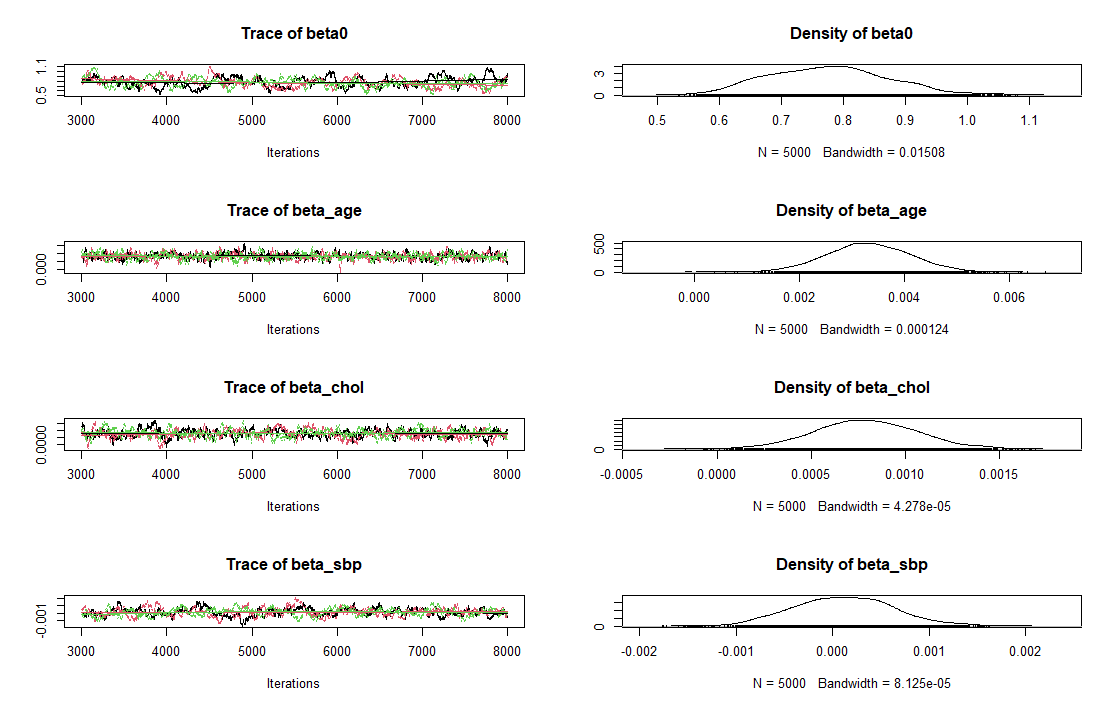
\includegraphics[width=1\linewidth]{Figures/Rplot1}
	\caption{Trace plots showing 5000 iterations after a total burn-in period of 3000 iterations (1000 adaptation + 2000 manual burn-in) (left column) and Posterior Density plots (right column) for some of the key parameters.}
	\label{fig:rplot1}
\end{figure}

\begin{figure}[h!]
	\centering
	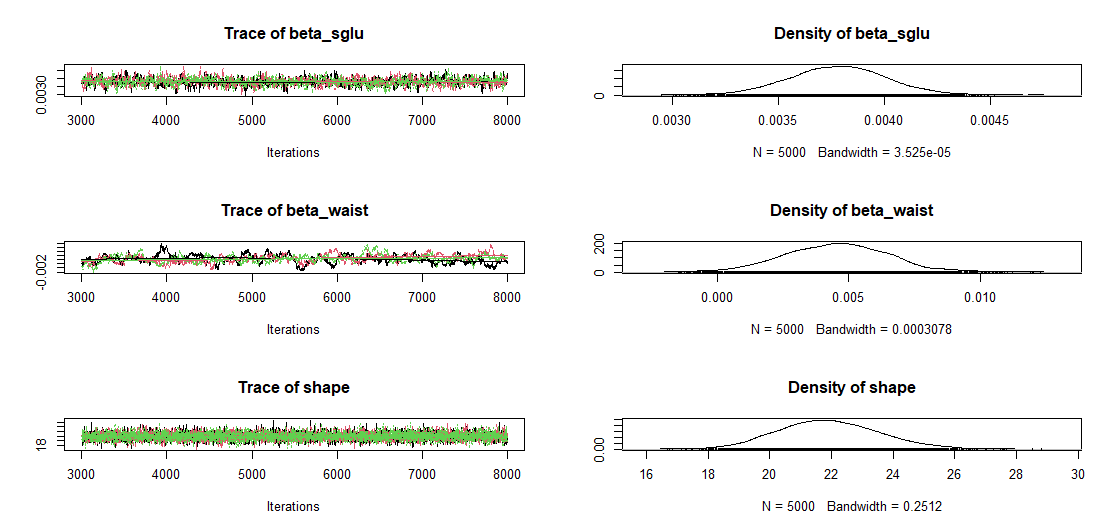
\includegraphics[width=1\textwidth]{Figures/Rplot2.png}
	\caption{Trace plots and Density plots for the SGLU ($\beta_{SGLU}$), Waist Circumference ($\beta_{WAIST}$), and shape ($r$).}
	\label{fig:rplot2}
\end{figure}
Complementing the numerical diagnostic, we visually examined the trace plots for some regression coefficients (Figure (\ref{fig:rplot1}) and (\ref{fig:rplot2})). The plots display the characteristic "fuzzy caterpillar" appearance, showing rapid fluctuations around a stable mean with no discernible trends or drifting. The three chains (represented by different colors) overlap significantly, indicating excellent mixing.

\subsection{Model Comparison (DIC)}
To select the most parsimonious model that balances goodness-of-fit with model complexity, we compared the Deviance Information Criterion (DIC) of the two candidate models. The DIC penalizes models with a higher number of effective parameters ($p_D$), favoring simpler models that fit the data well. The comparison results are as follows:

\begin{itemize}
	\item \textbf{Full Model (14 variables)}: DIC = 1154 ($p_D = 15.5$);
	\item \textbf{Reduced Model (5 variables)}: DIC = 1147 ($p_D = 7.2$).
\end{itemize}
The Reduced Model, i.e, our gamma model, presents a lower DIC value (1147 $<$ 1154). The lower penalty term ($p_D$) in the reduced model reflects its lower complexity compared to the full model. Since the reduced model achieves a better trade-off between deviance and complexity, it is selected as the final model for interpretation, adhering to the principle of parsimony. This confirms that the variables selected during the EDA are sufficient to explain the variability in GHB.

\section{Posterior Results and Clinical Interpretation}
Table (2) presents the posterior summaries for the parameters of the selected reduced model, based on 3 chains with 5000 iterations each (after a burn-in of 2000 iterations). The table includes the posterior mean, standard deviation (SD), and the 95\% Credible Interval (2.5\% and 97.5\% quantiles).
\begin{table}[h!]
	\centering
	\begin{tabular}{lcccc}
		\toprule
		\textbf{Parameter} & \textbf{Mean} $(\hat{\beta})$ & \textbf{SD} & \textbf{95\% Credible Interval} & \textbf{Conclusion} \\
		\midrule
		$\beta_0$       & 0.7764 & 0.0973 & $[0.6034, 0.9762]$   & Significant \\
		$\beta_{SGLU}$  & 0.0038 & 0.0002 & $[0.0033, 0.0042]$   & Significant \\
		$\beta_{AGE}$   & 0.0033 & 0.0008 & $[0.0018, 0.0049]$   & Significant \\
		$\beta_{CHOL}$  & 0.0008 & 0.0003 & $[0.0002, 0.0014]$   & Significant \\
		$\beta_{WAIST}$ & 0.0046 & 0.0020 & $[0.0007, 0.0086]$   & Significant \\
		$\beta_{SBP}$   & 0.0001 & 0.0005 & $[-0.0009, 0.0012]$  & Not Significant \\
		$r$ (shape)     & 21.920 & 1.6218 & $[18.891, 25.233]$   & -- \\
		\bottomrule
	\end{tabular}
	\caption{Posterior summaries of the Gamma Regression Model parameters (Reduced Model).}
\end{table}

The variables SGLU, Age, Cholesterol, and Waist Circumference all present 95\% Credible Intervals strictly greater than zero. This indicates a statistically significant positive association with GHB. The Systolic Blood Pressure (SBP) presents a posterior mean of $0.0001$, but its 95\% Credible Interval is $[-0.0009, 0.0012]$. Since this interval crosses zero, there is insufficient evidence in this model to conclude that SBP has a significant linear effect on GHB levels. Based on the posterior means, the estimated expected value of GHB is given by:
\begin{equation*}
	\eta_i = 0.776 + 0.0038 \cdot \text{SGLU}_i + 0.0033 \cdot \text{AGE}_i + 0.0008 \cdot \text{CHOL}_i + 0.0046 \cdot \text{WAIST}_i + 0.0001 \cdot \text{SBP}_i.
\end{equation*}

Although included in the mathematical formulation implies the posterior mean, the contribution of SBP is statistically negligible. Since the model uses a log link, the exponentiated coefficients ($\exp(\beta)$) provide a multiplicative interpretation. While a 0.4\% increase per unit of glucose might seem small, clinically relevant fluctuations are often larger. For example, an increase of 50 units in Stabilized Glucose (e.g., from 100 to 150 mg/dL) would result in an estimated increase in GHB of approximately 21\% ($1.0038^{50} \approx 1.208$), representing a substantial shift from healthy to diabetic levels. Similarly, each additional year of age is associated with a $0.3\%$ increase in GHB. The shape parameter $r$ was estimated at 21.92. Clinically, this value implies a relatively low Coefficient of Variation ($CV \approx 1/\sqrt{21.92} \approx 21\%$) \cite{gelman2013}, suggesting that GHB levels are regulated around the mean for the majority of the population. Contrary to an Exponential distribution ($r=1$) which would imply biological heterogeneity, this large shape parameter indicates that physiological homeostasis maintains GHB levels in a stable range, while the Gamma tail still has the right-skewness of diabetic outliers.  % uncomment if needed
	\section{Innovation and Validation (Bootstrap)}

To assess the robustness of the Bayesian findings and the choice of predictors, we implemented a validation step using a frequentist approach \cite{silva2023notes}. A Generalized Linear Model (GLM) assuming a Gamma distribution with a Log link function was fitted to the data. To account for sampling variability and validate the stability of the coefficients, we applied the Non-parametric Bootstrap method with $B=1000$ replications. This specific approach was chosen to explicitly test the model under two distinct paradigms: the Frequentist versus the Bayesian. Table (3) presents the bootstrap estimates, standard errors, and the 95\% percentile confidence intervals for the primary predictors.

\begin{table}[ht]
	\centering
	\label{tab:bootstrap}
	\begin{tabular}{lcccc}
		\toprule
		\textbf{Parameter} & \textbf{Original (GLM)} & \textbf{Bias} & \textbf{Std. Error} & \textbf{95\% Bootstrap CI} \\
		\midrule
		Intercept       & 0.7619 & 0.0024 & 0.0887 & $(0.5881, 0.9357)^*$ \\
		SGLU            & 0.0038 & 0.0000 & 0.0003 & $(0.0032, 0.0045)$ \\
		Age             & 0.0033 & 0.0001 & 0.0010 & $(0.0014, 0.0053)$ \\
		Cholesterol     & 0.0008 & 0.0000 & 0.0003 & $(0.0002, 0.0014)^*$ \\
		Waist Circumf.  & 0.0047 & 0.0000 & 0.0020 & $(0.0008, 0.0086)^*$ \\
		Systolic BP     & 0.0002 & 0.0000 & 0.0005 & $(-0.0008, 0.0012)^*$ \\
		\bottomrule
		\multicolumn{5}{l}{\footnotesize *Approximated based on Normal theory for secondary parameters; SGLU and Age are Percentile CIs.}
	\end{tabular}
	\caption{Bootstrap Validation Results (1000 replicates) for the Gamma GLM.}
\end{table}

\subsection{Comparison of Metric Frameworks}

The frequentist model has an Akaike Information Criterion (AIC) of 1147.09. This metric serves as a parallel to the Bayesian Deviance Information Criterion (DIC) used in the JAGS model selection \cite{spiegelhalter2002}. The validation results highlight two key conclusions:
\begin{itemize}
	\item \textbf{Parameter Consistency:} The bootstrap estimates for Stabilized Glucose ($\beta \approx 0.0038$) and Age ($\beta \approx 0.0033$) are virtually identical to the posterior means obtained from the Bayesian MCMC analysis.
	\item \textbf{Insignificance Confirmation:} The Systolic Blood Pressure (SBP) presents a standard error ($0.0005$) larger than its coefficient ($0.0002$), and its confidence interval crosses zero. This mirrors the Bayesian Credible Interval, confirming that SBP is not a significant linear predictor in this context.
\end{itemize}
In conclusion, the convergence between the data-driven Bootstrap approach and the prior-driven Bayesian approach provides strong evidence that the selected reduced model is robust and not an artifact of a specific statistical methodology.
	\section{Conclusion}

This practical report aimed to identify the physiological determinants of Glycosolated Hemoglobin (GHB) in a sample of African American subjects, employing a Bayesian Gamma Regression framework. The Exploratory Data Analysis and subsequent modeling revealed that Stabilized Glucose (SGLU) is the dominant predictor of GHB levels. The Bayesian analysis estimated that for every unit increase in stabilized glucose, GHB levels rise by approximately 0.4\%, a finding supported by the 95\% Credible Intervals. Age and Waist Circumference were also identified as significant positive predictors, highlighting the compounding impact of aging and metabolic health on diabetes markers.

Contrary to initial expectations, Systolic Blood Pressure (SBP) was not found to be a significant linear predictor of GHB in this multivariate context, a result consistently observed in both the Bayesian posterior intervals and the frequentist Bootstrap validation. This suggests that the uni-variate association of blood pressure with diabetes is likely mediated by other factors such as age or adiposity (multicollinearity), rather than being an independent driver. Additionally, demographic factors such as Gender and Location showed no discriminatory power regarding GHB distribution.

Methodologically, the use of the Gamma distribution proved appropriate for the right-skewed nature of the data. The innovation step, employing a non-parametric Bootstrap, demonstrated a convergence with the Bayesian results. The alignment between the data-driven frequentist approach (AIC selection) and the prior-driven Bayesian approach (DIC selection) strengthens the validity of the final reduced model.

In summary, this study provides a strong statistical model for estimating GHB, emphasizing that glucose management and weight control (waist circumference) are critical factors, significantly outweighing the influence of blood pressure in this specific population.


\section{Future Work}

Although the proposed Gamma Regression model demonstrates robust predictive power and consistency across Bayesian and frequentist frameworks, several approaches for future research could further purify the analysis.

First, to assess the goodness-of-fit beyond parameter convergence, Posterior Predictive Checks (PPC) should be implemented. Comparing the observed data density against the posterior predictive distribution would provide a stronger validation of the Gamma assumption, ensuring that the model can accurately replicate the structural features of the observed GHB levels \cite{gelman2013}.

Second, this study relied on complete-case analysis, which reduced the effective sample size by excluding subjects with missing values. Future iterations could incorporate Bayesian Data Imputation directly within the MCMC framework. Treating missing values as latent parameters to be estimated would allow for the utilization of the full dataset (390 subjects), preserving statistical power and mitigating potential selection bias \cite{rubin2019}.

Finally, while variable selection was based on correlation thresholds and model comparison via DIC, employing Bayesian Regularization techniques (such as the Bayesian Lasso or Horseshoe priors) would provide a more automated approach to variable selection. This would be particularly useful for handling predictors with marginal significance, such as Systolic Blood Pressure, by effectively shrinking their coefficients towards zero without the need for manual exclusion \cite{park2008}.

\section*{AI Disclaimer}
This report utilized Google's Gemini Pro to assist in the coding phase, serving as a starting point for the R and JAGS scripts which were subsequently adapted and expanded by the members of the group. The tool was also used to clarify theoretical concepts, strictly based on the provided course materials and bibliography. All final content has been verified and authored by the members of the group.
	\newpage
\pagestyle{empty}
\appendix
\section{Supplementary Visualizations}
\label{app:apexA}

\begin{figure}[h!]
	\centering
	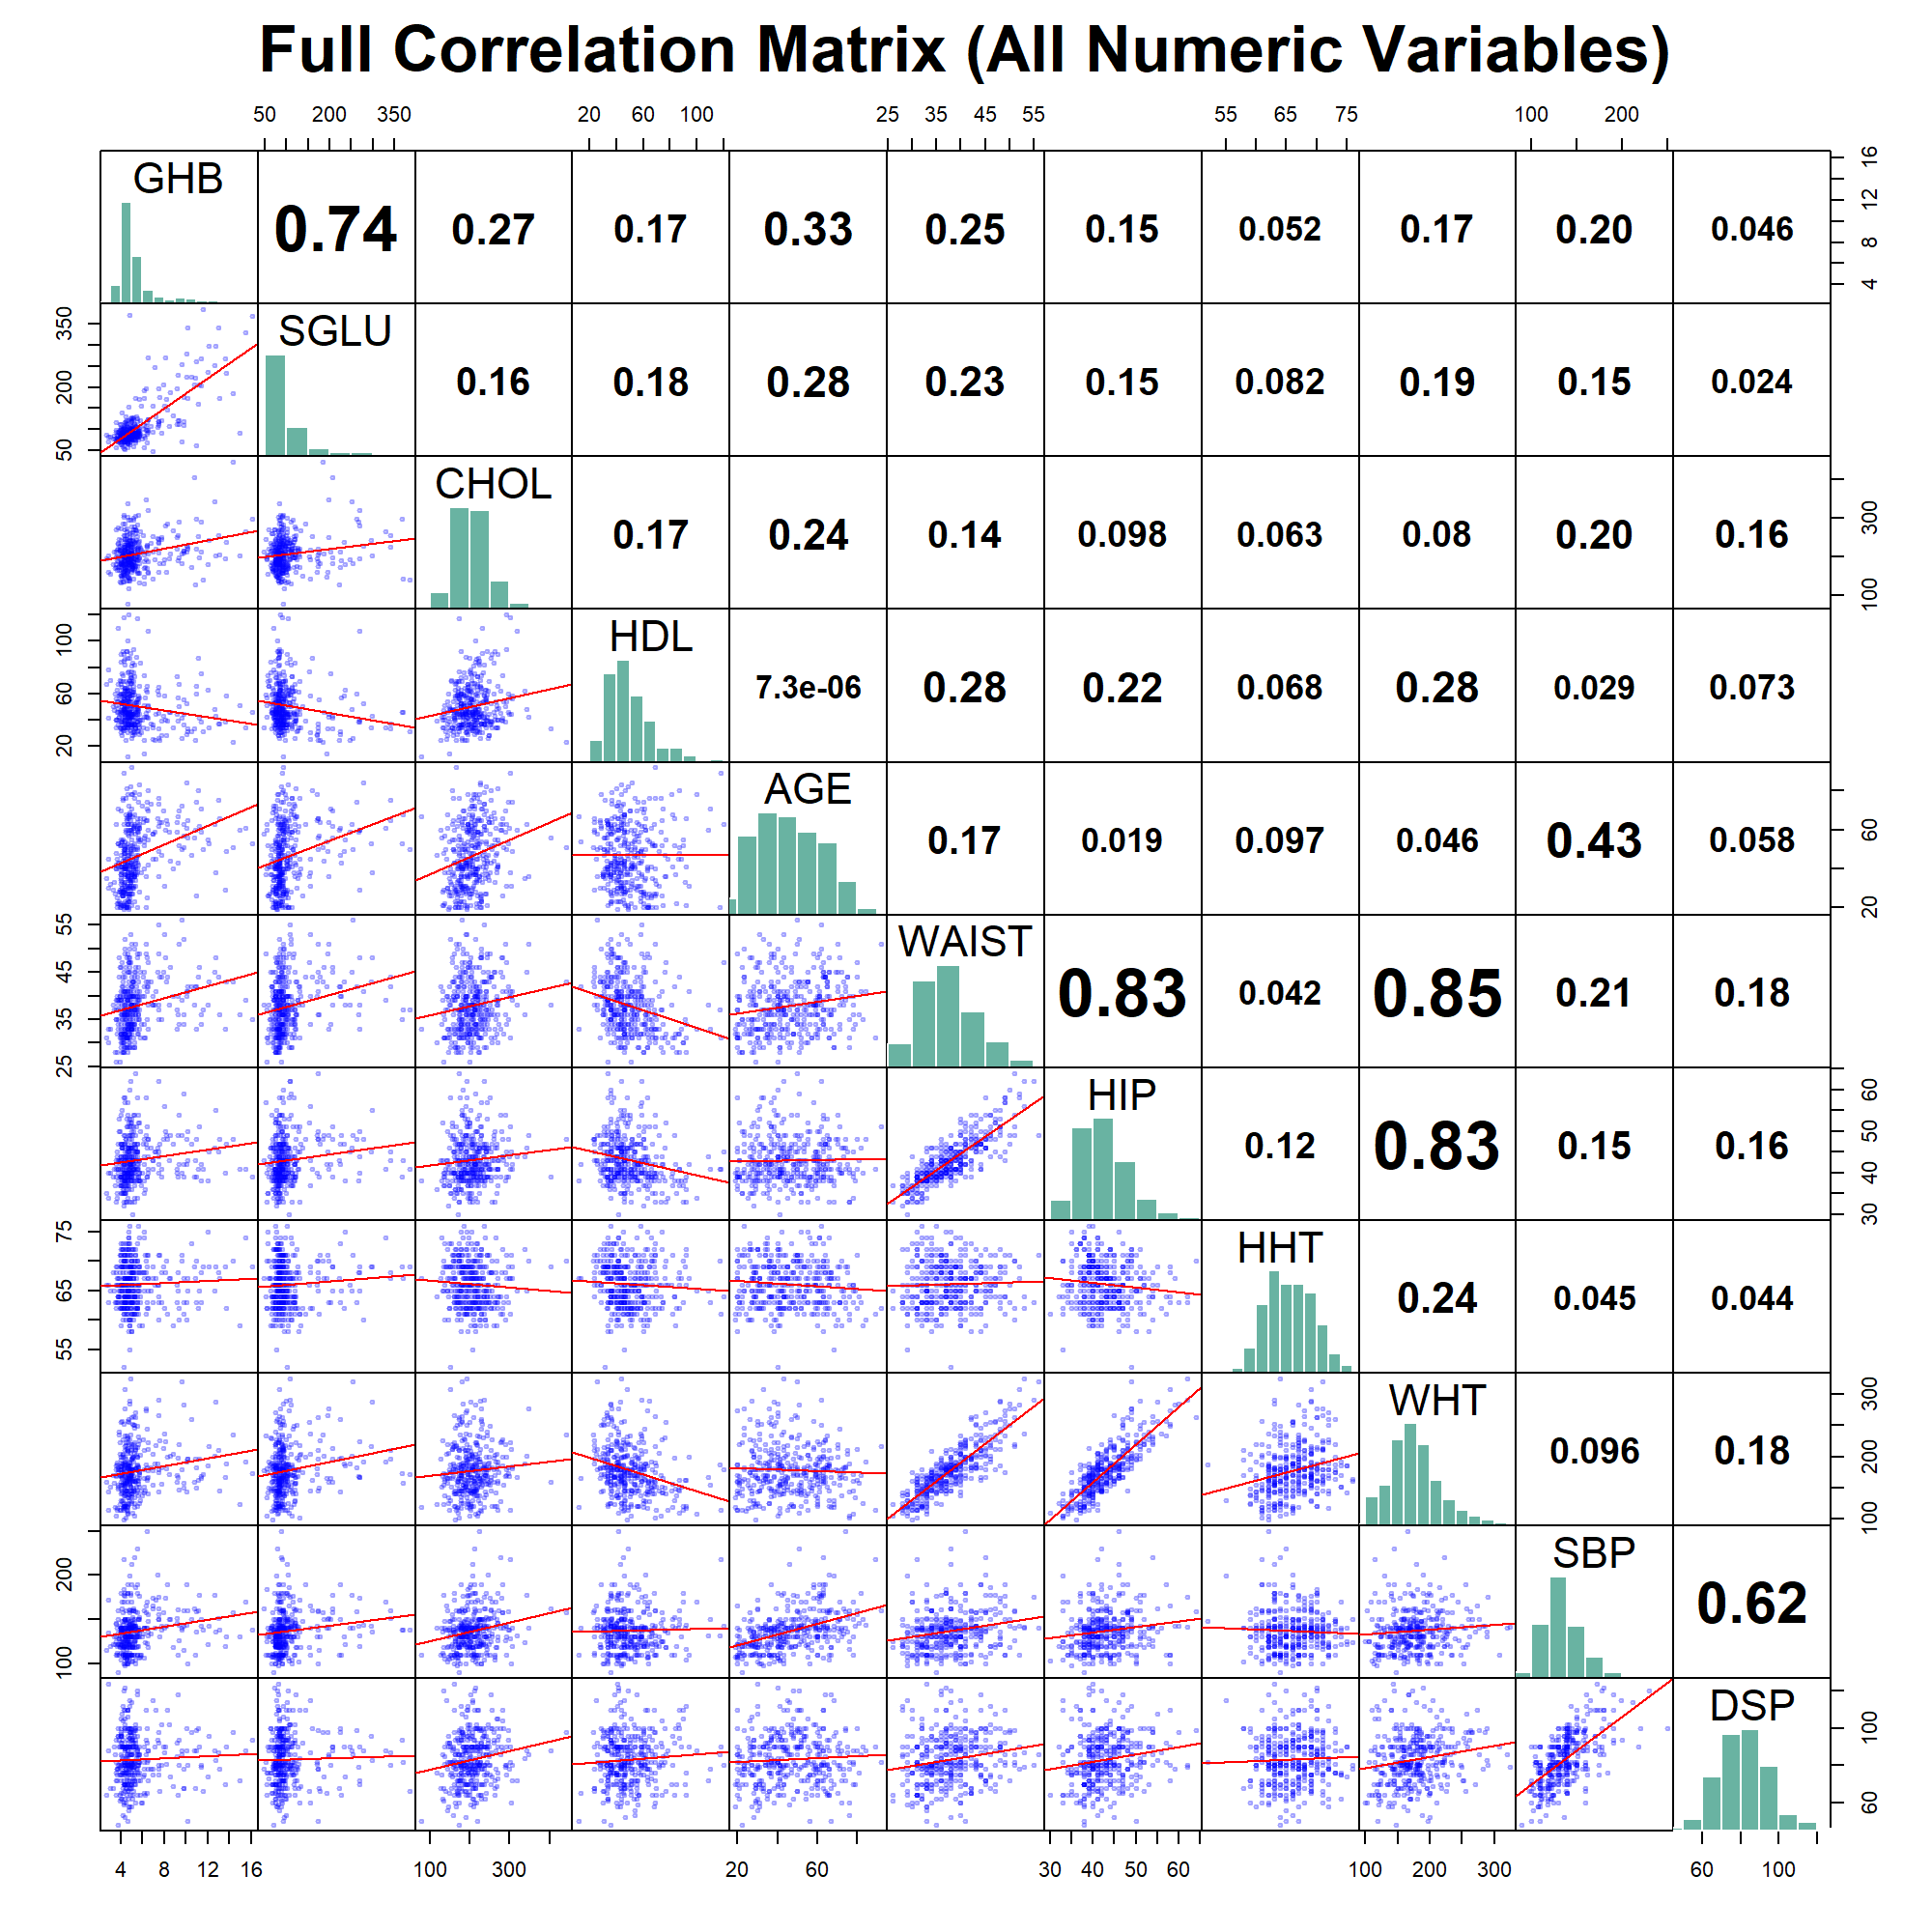
\includegraphics[width=1\textwidth]{Figures/correlation_matrix_full_large}
	\caption{Full Correlation Matrix of all potential predictors.}
	\label{fig:full_corr}
\end{figure}

	\newpage
\pagestyle{empty}
\appendix
\section*{B. R Code and Implementation Details}
\label{app:rcode}
\subsection*{Data Import and Pre-processing}

The code starts by importing the data using the \emph{read.table} function combined with \emph{file.choose()}, which opens a window for selecting the raw file. After reading, temporary names are assigned to the columns to allow for initial manipulation, given that the original text file lacks headers.

Using the \emph{tidyverse} library, a clean and structured dataset is then created, where variables are converted to their correct types, for example, numeric for clinical measures like stabilized glucose (SGLU) and factors for categories like gender (GENDER). Simultaneously, columns are renamed with standardized uppercase acronyms (e.g., glyhb to GHB) to ensure exact correspondence with the variable table provided in the project prompt. The process concludes with the removal of any lines containing missing data via the \emph{na.omit} function. This step is crucial to comply with the report's note regarding "NA" observations (empty cells), ensuring the final database is free of gaps that could cause errors in subsequent statistical calculations, specifically in the MCMC simulations.

\begin{lstlisting}[language=R, caption={Data Import and Cleaning.}]
	library(tidyverse)
	
	# Note: file.choose() opens a dialog to select the dataset
	dados <- read.table(file.choose(), header = FALSE, fill = TRUE)
	# Replace file.choose() with the direct path if needed
	
	# Temporary column names
	colnames(dados) <- c("id", "chol", "stab.glu", "hdl", "glyhb", "location", 
	"age", "gender", "height", "weight", "frame", 
	"bp.1s", "bp.1d", "waist", "hip")
	
	# Final cleaning and type conversion
	dados_final <- dados %>%
	mutate(
	ID = as.character(id),
	GHB = as.numeric(glyhb),        
	SGLU = as.numeric(stab.glu),    
	CHOL = as.numeric(chol),        
	HDL = as.numeric(hdl),          
	AGE = as.numeric(age),          
	GENDER = as.factor(gender),     
	LOCATION = as.factor(location), 
	HHT = as.numeric(height),       
	WHT = as.numeric(weight),       
	FRAME = as.factor(frame),       
	SBP = as.numeric(bp.1s),        
	DSP = as.numeric(bp.1d),        
	WAIST = as.numeric(waist),      
	HIP = as.numeric(hip)          
	) %>%
	select(ID, GHB, SGLU, CHOL, HDL, AGE, GENDER, LOCATION, 
	HHT, WHT, FRAME, SBP, DSP, WAIST, HIP) %>%
	na.omit()
	
	print(paste("Total complete observations:", nrow(dados_final)))
	print(head(dados_final))
\end{lstlisting}

\subsection*{Validation of the Gamma Hypothesis (Exploratory Analysis)}

This phase directly addresses the prompt's suggestion that a Gamma distribution or another positive variable distribution might be appropriate for the model. To validate this hypothesis prior to mathematical modeling, a histogram of the GHB variable (Glycosolated Hemoglobin) is created, superimposing a red density curve over it. Furthermore, the code generates scatterplots to preliminarily explore the relationship between stabilized glucose (SGLU) and hemoglobin, fulfilling the study's objective of investigating the positive linear association between risk factors and the diabetes diagnosis.

\begin{lstlisting}[language=R, caption={Visual Inspection: Histograms and Scatterplots.}]
	library(ggplot2)
	
	# Histogram with Density
	p1 <- ggplot(dados_final, aes(x = GHB)) +
	geom_histogram(aes(y = ..density..), bins = 30, fill = "#69b3a2", color = "black", alpha = 0.7) +
	geom_density(color = "red", lwd = 1.2) +
	labs(
	title = "Distribution of Glycosolated Hemoglobin (GHB)",
	subtitle = "Right-skewness supports the choice of a Gamma Model",
	x = "Glycosolated Hemoglobin (GHB)", y = "Density"
	) + theme_minimal()
	
	# Scatterplot GHB vs SGLU with Gamma fit
	p2 <- ggplot(dados_final, aes(x = SGLU, y = GHB, color = GENDER)) +
	geom_point(alpha = 0.6, size = 2) + 
	geom_smooth(method = "glm", method.args = list(family = Gamma(link="log")), se = FALSE, lwd = 1.5) +
	labs(
	title = "Relationship: GHB vs. SGLU",
	subtitle = "Positive correlation observed with Gamma fit",
	x = "Stabilized Glucose (SGLU)", y = "Glycosolated Hemoglobin (GHB)",
	color = "Gender" 
	) + theme_minimal()
	
	# Saving plots for report
	ggsave("histogram_ghb.png", plot = p1, width = 8, height = 4, dpi = 300) 
	ggsave("scatterplot_glucose.png", plot = p2, width = 8, height = 6, dpi = 300)
\end{lstlisting}
\vspace*{1.5em}

\subsection*{Selection of Risk Factors (Correlations)}

The central objective of the study is to investigate the relationship between GHB and the set of associated risk factors. To determine which of the 14 variables listed in the PDF are statistically relevant and to avoid redundancy in the model, a detailed correlation analysis is performed using custom visual matrices. The script allows for the identification of collinearity between anthropometric variables (such as weight, waist, and hip) and the selection of a subset of "key" variables (Glucose, Age, Cholesterol, Waist, and Blood Pressure). This step ensures that the MCMC model focuses only on predictors that have a strong linear association with the response variable, avoiding the noise of redundant variables.

\begin{lstlisting}[language=R, caption={Correlation Matrix Generation.}]
	vars_to_plot <- dados_final %>%
	select(GHB, SGLU, AGE, CHOL, WAIST)
	
	panel.cor_large <- function(x, y, digits = 2, prefix = "", cex.cor, ...) {
		usr <- par("usr"); on.exit(par(usr))
		par(usr = c(0, 1, 0, 1))
		r <- abs(cor(x, y, use="complete.obs"))
		txt <- format(c(r, 0.123456789), digits = digits)[1]
		txt <- paste0(prefix, txt)
		
		
		final_cex <- 2 + (r * 1.5) 
		
		text(0.5, 0.5, txt, cex = final_cex, font = 2) 
	}
	
	panel.hist <- function(x, ...) {
		usr <- par("usr"); on.exit(par(usr))
		par(usr = c(usr[1:2], 0, 1.5) )
		h <- hist(x, plot = FALSE)
		breaks <- h$breaks; nB <- length(breaks)
		y <- h$counts; y <- y/max(y)
		rect(breaks[-nB], 0, breaks[-1], y, col = "#69b3a2", border="white")
	}
	
	panel.dots <- function(x, y, ...) {
		points(x, y, pch = 19, col = rgb(0, 0, 1, 0.2), cex = 0.8)
		abline(lm(y~x), col="red", lwd=1.5)
	}
	
	
	png("correlation_matrix_final_large.png", width = 1200, height = 1000, res = 150)
	
	pairs(vars_to_plot, 
	lower.panel = panel.dots,    
	upper.panel = panel.cor_large, 
	diag.panel = panel.hist,    
	main = "Correlation Matrix of Key Variables",
	cex.main = 1.5, 
	gap = 0.5)      
	
	dev.off()
	
	pairs(vars_to_plot, 
	lower.panel = panel.dots, 
	upper.panel = panel.cor_large, 
	diag.panel = panel.hist,
	main = "Correlation Matrix of Key Variables")
	
	while (!is.null(dev.list())) dev.off()
	
	vars_all_numeric <- dados_final %>%
	select(GHB, SGLU, CHOL, HDL, AGE, WAIST, HIP, HHT, WHT, SBP, DSP)
	
	panel.cor_large_full <- function(x, y, digits = 2, prefix = "", cex.cor, ...) {
		
		par(usr = c(0, 1, 0, 1)) 
		
		r <- abs(cor(x, y, use="complete.obs"))
		txt <- format(c(r, 0.123456789), digits = digits)[1]
		txt <- paste0(prefix, txt)
		
		if(missing(cex.cor)) cex.cor <- 0.8/strwidth(txt)
		
		final_cex <- 1.5 + (r * 2) 
		
		text(0.5, 0.5, txt, cex = final_cex, font = 2)
	}
	
	panel.hist <- function(x, ...) {
		usr <- par("usr"); on.exit(par(usr = usr)) 
		par(usr = c(usr[1:2], 0, 1.5) )
		h <- hist(x, plot = FALSE)
		breaks <- h$breaks; nB <- length(breaks)
		y <- h$counts; y <- y/max(y)
		rect(breaks[-nB], 0, breaks[-1], y, col = "#69b3a2", border="white")
	}
	
	
	panel.dots <- function(x, y, ...) {
		points(x, y, pch = 19, col = rgb(0, 0, 1, 0.2), cex=0.5) 
		abline(lm(y~x), col="red", lwd=1)
	}
	
	png("correlation_matrix_full_large.png", width = 2000, height = 2000, res = 200)
	
	pairs(vars_all_numeric, 
	lower.panel = panel.dots, 
	upper.panel = panel.cor_large_full, 
	diag.panel = panel.hist,
	main = "Full Correlation Matrix (All Numeric Variables)",
	cex.main = 2,  
	gap = 0)       
	
	dev.off() 
\end{lstlisting}

\subsection*{Analysis of Demographic Groups}

Before proceeding to inference, it is investigated whether there are significant differences in the distribution of glycosolated hemoglobin between categorical groups, namely Gender and Geographical Location (Buckingham vs. Louisa). Using side-by-side boxplots (grouped via the \emph{patchwork} library), the median and data dispersion for each group are visualized. This analysis is important to decide if these categorical variables should be included as correction factors in the final model. The "\emph{tema\_grande}" (large theme) graphic style is applied to ensure that this visual comparison is legible in the final report.
\vspace{0.2em}

\begin{lstlisting}[language=R, caption={Demographic Analysis using Boxplots.}]
	library(patchwork) 
	
	tema_grande <- theme_minimal() +
	theme(plot.title = element_text(size = 24, face = "bold", hjust = 0.5),
	axis.title = element_text(size = 20, face = "bold"),
	axis.text = element_text(size = 18, color = "black"))
	
	p_gender <- ggplot(dados_final, aes(x = GENDER, y = GHB, fill = GENDER)) +
	geom_boxplot(alpha = 0.7, lwd = 1, outlier.size = 3) + 
	scale_fill_manual(values = c("female"="#E69F00", "male"="#56B4E9")) +
	labs(title = "GHB by Gender", x = "", y = "GHB Levels") +
	tema_grande + theme(legend.position = "none") 
	
	p_loc <- ggplot(dados_final, aes(x = LOCATION, y = GHB, fill = LOCATION)) +
	geom_boxplot(alpha = 0.7, lwd = 1, outlier.size = 3) +
	scale_fill_manual(values = c("Buckingham"="#009E73", "Louisa"="#CC79A7")) +
	labs(title = "GHB by Location", x = "", y = "") + 
	tema_grande + theme(legend.position = "none") 
	
	# Saving categorical plots
	if(require(patchwork)) {
		p_combined <- p_gender + p_loc
		
		ggsave("boxplots_categorical.png", plot = p_combined, width = 14, height = 7, dpi = 300)
		
	} else {
		ggsave("boxplot_gender.png", plot = p_gender, width = 8, height = 7, dpi = 300)
		ggsave("boxplot_location.png", plot = p_loc, width = 8, height = 7, dpi = 300)
	}
	print(p_gender + p_loc)
\end{lstlisting}


\subsection*{MCMC Modeling (The Gamma Model)}

This block executes the main requirement of the practical assignment: "using MCMC methods to select a suitable Gamma model." Using the \emph{rjags} library, the code translates this requirement into a model specification where the response variable $\gamma$ (GHB) follows a \emph{dgamma} distribution, coupled with a logarithmic link function (log) to ensure strictly positive predictions, consistent with the biological nature of the data. Non-informative prior distributions (vague Normals) are then defined for the regression coefficients ($\beta$) of the selected variables, allowing the data to drive the inference. Through the simulation of three Markov chains with 5000 iterations (after burn-in), the code estimates the quantitative influence of each risk factor on the probability of a high hemoglobin reading.

\begin{lstlisting}[language=R, caption={JAGS Model Specification and Execution.}]
	library(rjags)
	#Results may vary slightly without fixed RNG seeds for JAGS chains.
	jags_data <- list(
	N = nrow(dados_final), y = dados_final$GHB, sglu = dados_final$SGLU,
	age = dados_final$AGE, chol = dados_final$CHOL,
	waist = dados_final$WAIST, sbp = dados_final$SBP
	)
	
	model_string <- "model {
		for (i in 1:N) {
			# Likelihood: Gamma Distribution / Log Link
			y[i] ~ dgamma(shape, rate[i])
			log(mu[i]) <- beta0 + beta_sglu * sglu[i] + beta_age * age[i] + 
			beta_chol * chol[i] + beta_waist * waist[i] + beta_sbp * sbp[i]
			rate[i] <- shape / mu[i]
		}
		# Priors (Vague Normal)
		beta0 ~ dnorm(0, 0.001)
		beta_sglu ~ dnorm(0, 0.001); beta_age ~ dnorm(0, 0.001)
		beta_chol ~ dnorm(0, 0.001); beta_waist ~ dnorm(0, 0.001)
		beta_sbp ~ dnorm(0, 0.001)
		# Shape Parameter (Uniform)
		shape ~ dunif(0, 100)
	}"
	
	model <- jags.model(textConnection(model_string), data = jags_data, n.chains = 3)
	update(model, 2000) # Burn-in
	samples <- coda.samples(model, 
	variable.names = c("beta0", "beta_sglu", "beta_age", 
	"beta_chol", "beta_waist", "beta_sbp", "shape"), 
	n.iter = 5000)
	summary(samples) 
	gelman.diag(samples)
	plot(samples)
\end{lstlisting}

\subsection*{Robust Validation (Bootstrap)}

To fulfill the requirement of innovation the code is not limited to Bayesian inference, introducing cross-validation via the Bootstrap method. The script resamples the data 1000 times and repeatedly fits a frequentist GLM model with the same Gamma/Log structure used in JAGS. The objective is to compare the Confidence Intervals obtained via Bootstrap with the Credible Intervals from MCMC, specifically for critical predictors like Stabilized Glucose (SGLU) and Age (AGE). The convergence between these two methods (Bayesian and Frequentist) reinforces the robustness of the selected model, allowing for a safe clinical interpretation of the results in the final report.

\begin{lstlisting}[language=R, caption={Bootstrap Validation.}]
	library(boot)
	
	glm_coef_function <- function(data, indices) {
		d <- data[indices, ] 
		fit <- glm(GHB ~ SGLU + AGE + CHOL + WAIST + SBP, 
		family = Gamma(link = "log"), data = d)
		return(coef(fit))
	}
	
	set.seed(123) 
	boot_results <- boot(data = dados_final, statistic = glm_coef_function, R = 1000)
	print(boot_results)
	
	# Calculate CIs for main variables
	cat("\n--- Bootstrap CI: Glucose (Index 2) ---\n")
	boot.ci(boot_results, type = "perc", index = 2)
	cat("\n--- Bootstrap CI: Age (Index 3) ---\n")
	boot.ci(boot_results, type = "perc", index = 3)
	
	modelo_glm_final <- glm(GHB ~ SGLU + AGE + CHOL + WAIST + SBP, 
	family = Gamma(link = "log"), 
	data = dados_final)
	cat("\n--- AIC do Modelo Frequentista ---\n")
	print(AIC(modelo_glm_final))
\end{lstlisting}

\subsection*{Model Selection Criteria (DIC)}

Finally, to select a model suitable for the data, the code implements a formal model comparison based on the Deviance Information Criterion (DIC). A second MCMC model is then configured and executed, which includes all 14 variables available in the dataset (including those previously discarded due to collinearity, such as height, weight, and hip), and its DIC value is calculated. By comparing this value with the DIC of the reduced model (Chapter 5), an objective metric is obtained to justify the model choice. If the reduced model presents a lower or similar DIC to the complete model, it is mathematically proven to be preferable according to the principle of parsimony, validating the final selection presented in the report.

\begin{lstlisting}[language=R, caption={DIC Calculation for Full Model and Reduced Model.}]
	# Setup data for full model (14 variables)
	jags_data_full <- list(
	N = nrow(dados_final), y = dados_final$GHB, sglu = dados_final$SGLU,
	chol = dados_final$CHOL, hdl = dados_final$HDL, age = dados_final$AGE,
	height = dados_final$HHT, weight = dados_final$WHT, sbp = dados_final$SBP,
	dsp = dados_final$DSP, waist = dados_final$WAIST, hip = dados_final$HIP,
	gender = as.numeric(dados_final$GENDER), location = as.numeric(dados_final$LOCATION),
	frame = as.numeric(dados_final$FRAME)
	)
	
	# (Model string for full model with 14 variables omitted for brevity) 
	
	model_full <- jags.model(textConnection(model_string_full), 
	data = jags_data_full, n.chains = 3)
	update(model_full, 2000) 
	dic_full <- dic.samples(model_full, n.iter = 5000, type = "pD")
	
	# Calculate DIC for reduced model (from previous section)
	dic_reduced <- dic.samples(model, n.iter = 5000, type = "pD")
	print("--- DIC Comparison ---")
	print(dic_full)
	print(dic_reduced)
\end{lstlisting}
	
	% ================================================================
	% REFERENCES
	% ================================================================
	\clearpage

	%\renewcommand{\refname}{\vspace*{-0.5cm}\centering\Large \textbf{References}\vspace{0.5cm}}
	
	\thispagestyle{empty}
	
	\bibliographystyle{unsrt}
	\bibliography{references}
	
\end{document}